\documentclass[a4paper,14pt]{extreport}
\newcommand\tab[1][1cm]{\hspace*{#1}}
% packages to support Cyrillic fonts, needed to write abstracts
\usepackage[T2A]{fontenc} 
\usepackage[utf8]{inputenc} 
\usepackage[russian,english]{babel}
\usepackage{csquotes}
\usepackage{graphics}
\usepackage{graphicx}
\usepackage{hyperref}
\usepackage{booktabs}
\usepackage{cleveref}
\usepackage{tabu}
\usepackage{enumitem,xcolor}
\usepackage{hyperref,cleveref}
\usepackage[numbers]{natbib}
\hypersetup{
  colorlinks = true,
  linkcolor = blue
}
%
\usepackage[utf8]{inputenc} 
\usepackage[russian,english]{babel}
\usepackage{csquotes}

% usual packages
\usepackage[left=30mm, right=10mm, top=20mm, bottom=20mm]{geometry}

\usepackage{graphicx} % to add figures
\graphicspath{{figures/}}

\usepackage{hyperref} % to add clickable contents menu

\usepackage[style=numeric]{biblatex}
\addbibresource{bibliography.bib}

\usepackage{blindtext}
%


% usual packages
\usepackage[left=30mm, right=10mm, top=20mm, bottom=20mm]{geometry}

\usepackage{graphicx} % to add figures
\graphicspath{{figures/}}

\usepackage{hyperref} % to add clickable contents menu

\usepackage[style=numeric]{biblatex}
\addbibresource{bibliography.bib}

\usepackage{blindtext}

% the following three definitions are to be changed by student
\def\myauthor{
Aigerim Mazhtay \\
Aray Turgyn\\
Magzhan Kozhakhmet  \\
Saida Seitzhan 
}
\def\mycoach{Ualikhan Sadyk} % coach, adviser etc.
\def\mytitle{Discipline management system} % title
\def\mydegree{Bachelor in Computer Systems and Software}
\def\mydegreecode{6B06102}


% preamble ends here

\begin{document}
    % don't touch these two lines :)
    
    \begin{titlepage}
\begin{center}
\large
Ministry of Education and Science of the Republic of Kazakhstan

Suleyman Demirel University

\vspace{1cm}
\begin{figure}[h]
    \centering
    
\includegraphics[scale=0.5]{sdu_only}
\end{figure}

\vspace{1cm}
\Large
\myauthor

\vspace{1cm}
\Large
\textbf{\mytitle}

\vspace{1cm}
\large
A thesis submitted for the degree of

\mydegree

(degree code: \mydegreecode)

\vfill
Kaskelen, 2022

\end{center}
\end{titlepage}

    \newpage
\pagestyle{empty}

\begin{center}
\large
Ministry of Education and Science of the Republic of Kazakhstan

Suleyman Demirel University

Faculty of Engineering and Natural Sciences

\vspace{2cm}
\textbf{\mytitle}

\vspace{1cm}
\large
A thesis submitted for the degree of

\mydegree

(degree code: \mydegreecode)

\vspace{2cm}
Author: \textbf{\myauthor}

\vspace{2cm}
Supervisor: \textbf{\mycoach}

\vspace{2cm}
Dean of the faculty:

\textbf{Assist. Prof. Azamat Zhamanov}


\vfill
Kaskelen, 2022
\end{center}

    
    % edit abstracts
    \newpage
\pagestyle{plain}

{\selectlanguage{english}
\begin{center}
    \Large
    \textbf{Abstract}
\end{center}
\par "Your patriotism is not measured by what your country can do for you. It's all about what you can do for your country for your own benefit and for the benefit of unborn generations!” as Israelmore Ayivor said, this is the phrase that forced us to create a platform for the favor of our country's young generation. We live in the new age of technology, where each of us aspire to achieve one's goal. The purpose of the research is the realization of an educational platform combined with national aspects. The platform which is adjusted  with one of the most efficient approaches of managing online education \cite{song2004improving}. Methods of gathering and processing information, including expert interviews and questionnaires were used in the study. The analysis of the system of online education in our country and abroad provides reasons to assume that the experience, assembled in the field of online learning today, paves the way for the formation of the new  format of distance learning.\cite{khan2011let}
This research outlines the online platform requirements, methods and tools, challenges faced during implementation, and possible future iterations of our course.
}


    \newpage
\pagestyle{plain}

{\selectlanguage{kazakh}
\begin{center}
    \Large
    \textbf{Аңдатпа}
\end{center}
\par «Сіздің патриотизміңіз еліңіздің сіз үшін не істей алатынымен өлшенбейді. Мұның бәрі өз игілігің үшін және туылмаған ұрпақтың игілігі үшін елің үшін не істей аласың!». Израильмор Айивор айтқандай, бұл бізді еліміздің жас ұрпақтарының игілігі үшін платформа құруға мәжбүрлеген сөз тіркесі. \\
Зерттеудің мақсаты - біз анықтағандай, бар платформа тәжірибелері мен практикалық ұсыныстарды пайдалана отырып, қашықтықтан білім беруді басқарудың ең тиімді тәсілдерінің бірі \parencite{song2004improving} анықтау және жүзеге асыру. Зерттеу барысында ақпаратты жинау және өңдеу әдістері, оның ішінде сарапшылар сұхбаты мен сауалнамалар қолданылды. Еліміздегі және шетелдегі қашықтықтан білім беру жүйесін талдау бүгінгі күні қашықтықтан оқыту саласында жинақталған тәжірибе қашықтан оқытудың жаңа форматын қалыптастыруға жол ашады деп болжауға негіз береді.\parencite{khan2011let}
Бұл зерттеу виртуалды сыныптың тарихын, нақты талаптарды, іске асыру кезінде кездесетін қиындықтарды және біздің курстың мүмкін болатын итерацияларын сипаттайды.
}

    \newpage
\pagestyle{plain}

{\selectlanguage{russian}
\begin{center}
    \Large
    \textbf{Аннотация}
\end{center}
\par «Ваш патриотизм не измеряется тем, что ваша страна может сделать для вас. Все дело в том, что вы можете сделать для своей страны во благо себе и во благо будущих поколений!» как сказал Исраэльмор Айвор, именно эта фраза заставила нас создать платформу в пользу молодого поколения нашей страны.
Целью исследования является выявление и реализация одного из наиболее эффективных подходов \parencite{song2004improving}, как мы определили, управления дистанционным образованием с использованием существующего опыта платформы и полученных нами практических предложений. В исследовании использовались методы сбора и обработки информации, в том числе экспертные интервью и анкетирование. Анализ системы дистанционного образования в нашей стране и за рубежом дает основания предполагать, что опыт, накопленный в сфере дистанционного обучения сегодня, прокладывает путь к формированию нового формата дистанционного обучения.\parencite{khan2011let}
В этом исследовании описывается история виртуального класса, конкретные требования, проблемы, возникающие при реализации, и возможные будущие итерации нашего курса.
}

    \tableofcontents
    
    % edit your chapters
    \chapter{Introduction}\label{ch:intro}
%these sections are optional, up-to the author
We know that Kazakh people are well-endowed from their own nature. They have huge potential to acquire new skills in short stretch of time, they can pretend for the bright future if they keep up on progressing and developing their national values. However, we shouldn't leave off just with national values. In order to be able to offer something valuable to the regional and global markets nation and every person comprising the nation should be competitive. Competitive not in terms of only material goods, but also in terms of knowledge, intellectual products and quality of human resources. 

Thus, we aimed to create a platform which will either contribute to the significant area of nation's development and help to uplift national spirit in the education sector. The project which will make learners look over gaining knowledge from the other angle, through other lens. The platform that will be in use of every school children's academic and daily life.

We came up with an idea to create an Educational Learning Management Platform, which enables students to track their own progress and to prioritize tasks. I can say this is our main foremost attribute. Why did we focus on it so much? Because, our progress, our accomplishments - are what give us energy. Energy to conquest, energy to achieve more accomplishments, energy to do significant realizations. This is an idea that comes from well-known Kaizen planning system. According to this system we should see our all life-through performances, acts, deeds in a visual desk.\cite{singh2009kaizen} Thus, we built on function into our product, which is called progress tracking.

Moreover, according to the article written by Richelle V. Adams1, Erik Blair published in journal "Sage" \ref{ch:Ref}: successful time management is associated with greater academic performance and lower levels of anxiety in students. Consequently, we decided to add some features for time management. 

It is difficult to overestimate the opportunities that online education systems offer to students of our time. Equal access to information, low barriers to knowledge acquisition, mobility and constantly updated material are the main advantages of the platforms. And nowadays there are a lot of online courses and platforms for use in universities and schools. 

Online educational platforms are able to form independence and cooperation skills in the process of building online network interactions, which is beneficial for a modern person, since these skills are valued much more in the process of modern communication than the discipline and competition developed by classical educational models. 

The idea of our platform is that it provides the school community with 
1. the platform that will make school learners remember that they're citizens of Kazakhstan, by adding national patterns in national style.
2. the platform enriched with features that didn't exist in educational school platforms before, where each task/project is supported by extension in the form of multi-level tasks, the completion of which contribute to consistent and systematic learning of skills. 

It is interesting to note the fact that 93\% of studies found at least one engagement dimension \& 50\% at least one disengagement dimension in the learning approach was found according to the research held in the University College London \cite{bond2020facilitating}. And also highlighting the claim that teacher-created videos are more likely to lead to task completion & overall engagement is also worth it \cite{bond2020facilitating}. So, from this we get an  assumption that there should be an update or transformation in learning approach at schools. Because, school is the place where children make the first impression about gaining education.  

We hope to contribute to youth development by facilitating their learning process, making it more creative and engaging; and accustoming them to plan their activities, goals, to keep them motivated by providing them with motivational citates while they're using our product. In conclusion, we want all Kazakh children to achieve their goals, to set clear expectations for themselves, always to be full of beans. Overall, we expect them to contribute to the development of our motherland and to be an honest, well-educated citizen. 

\section{Problem statement}
In our country we don't have a platform for school staff, with new functionalities, new design,  For instance, at the moment there are platforms for universities, where students can see the whole content/topics that will be taught during the study of the subject in advance. But school learners lacking this opportunity. This is just one drop of a problem that we found out during our research. Analysis showed us that there were some cases even which represent a reputational risk.\\ 
Moreover, there is a new trend, according to which cartoons, films, accessories, clothes, comics are produced in a way they contribute to our national values, by creating their own modern kazakh style. Furthermore, the circumstances of our national values are hanging in the balance nowadays, so there should be a place for maintaining Kazakh style in educational platforms as well.\\
Before creating our project we defined specific range of questions that arose in our minds. \\
\textbf{What additional functions do teachers and children need during the work with online platforms? }\\
\textbf{What functions are hard to be found in the online education environment?}\\
\textbf{How to improve the level of productivity of school children?}\\
We need to build a platform that will bridge the gaps in online learning environment at schools of Kazakhstan. 
\newpage
\section{Aims and Objectives}
\subsubsection{Aim:}
Organize learning system in a new functional way by maintaining national style .
\subsubsection{Objectives: }
Investigations on existing platforms will be performed.\\
Time tracker will be created.\\
Secure plagiarism checker will be developed. \\
User friendly webpage in user friendly, slightly national design will be built. \\
Downsides of existing platforms will be added to our's as strengths.
\section{Thesis Outline}
Theme: "Subject management platform: Easy Mektep". \\
The main goal of the diploma project was to solve some problems of virtual education system of Kazakhstan. To tackle this, we brainstormed, made research and created a platform with essential, in demand functions which were acknowledged by questionnaire results.\\
The diploma project includes an introduction, problem statement, requirements, planning, methodologies, final conclusion, future iterations, list of references and literature.\\
Keywords: distance learning, online classes, MySQL, PHP, Anti-plagiarism, PYTHON, sklearn, cosine-similarity.

    \chapter{Background review}\label{ch:A}
\section{Product description}
Easy Mektep is a subject management platform developed by our team in favour of schoolchildren, where schoolchildren can easily organize, complete assigned tasks and track their own progress, control one's time consuming habits. Also, it is a platform, where teachers can create classes and upload assignments for students and check them. In addition, due to the plagiarism checker feature, teachers are able to find cheaters and see overall statistics on children's works' uniqueness(antiplagiarism).  \\
The platform should be slightly styled with national patterns, in order to preserve our national style. 
The site presents a multi-level system for organising the lesson content. The lessons were developed with the use of the task-based learning approach. While completing a task of a certain priority, a student is involved in the active cognitive process. Each task provides a short introductory material and bonus announcement system which helps student to effectively concentrate his knowledge on the task and contributes to successful completion of the task.
\section{User requirements }
\vspace{0.4cm}
\subsubsection{To test whether a user story is well formed, we applied the acronym INVEST \cref{app:B}.\cite{buglione2013improving}}
\vspace{1cm}
\large \textbf{User stories}
\vspace{0.4cm}\\
* As a new user, I want to sign up using my existing Google account so that I don't have to keep track of another account.

* As an existing student, I want to see all my tasks, so that I don't miss any of them.

* As a student, I want to break down assigned tasks, and prioritize them, so that I could work effectively.

* As a teacher, I want to create classes, add students to them, and assign them tasks/projects.

* As a teacher, I want to see statistics on plagiarism, to make sure that evaluating process is fare. 

* As a teacher, I want to see students' progress for specific data range. 

* As a student, I want to see time I spent on particular task, so that I can manage my energy and distribute my time wisely.

* As a student, I want to easily use it from any gadget.

* As a student, I want to control your time spent on  studying.
\section{Product Requirements Document - PRD} \label{sec:PRD}
Product should solve outstanding problems in education like lack of motivation, not receiving timely feedback, not receiving clear instructions or expectations. \cref{ch:Ref}\\
Students should be able to understand what advantages the completion of task will provide them. \\
Exam dates, day offs, and other special calendar events should be clearly visible.\\
Teacher info for contacting should be always on hand.\\
Platform should be trustworthy.\\
Students can upload their works.\\
The platform website must be responsive: work well and look good on all screen sizes.\\
The product should have two roles: students and teachers, in order to reduce misunderstandings between a teacher and a student while grading and handing in assignments.\\
Teachers can upload their assignments for students and check them. \\
Teachers can check works for plagiarism.
Students should have answers for the following questions:\\
* What type of material you’ll be covering?\\
* How each type of assignment will be graded?\\
* What are the deadlines?\\

    \section{Functional requirements}\vspace{0.3cm}
The system shall have authentication measures at inbound network connection.\\
The platform should have an adaptive website which allows users to easily use it from any gadget.\\
Passwords should be created/recreated in accordance with system requirements.\\
The system shall support authentication based on device local authority.\\
The system shall support multiple authentication approaches at the same time.\\
The system must make sure the database entrance is executed using parameterized store procedures to allow all table approaches to be cancelled.\\
In more detail in \hyperlink{thistable}{this page}.
\section{Non-functional requirements}
Usability: End user satisfaction. \\
Security: the product must cover basic security requirements, such as: \\
a) Authentication and password management\\
b) Authorization and role management.\\
c) Login with Session \\
Portability: the same quality should be preserved on different devices\\
Reliability: Time between critical failures\\
Performance: The application must be able to support at least 50 simultaneous users.\\


    \chapter{Methodology}\label{ch:B}
\section{Planning}
We agreed on working with the Agile methodology. We love working with this way of approaching the project development, because it allows us to be flexible and don't be afraid of changes that we can face in the future. Furthermore, the Agile methodology has several advantages over traditional ways of developing a software. As, shown below: \cref{ch:Ref} \newline
\large \textbf {4 Values of Agile}\newline
Individuals and interactions over processes and tools.\\
Working software over comprehensive documentation.\\
Customer collaboration over contract negotiation.\\
Responding to change over following a plan.\\
\vspace{0.2cm}
\newline 1-scrum: define roles, choose an idea, plan sprints, prioritize our project.
\newline 2-scrum: creating a sketch of the site design model, finalizing the idea with improvements, general analysis of other educational platforms.
\newline 3-scrum: making adjustments to the functionality, its expansion. Make up the finished design. Setting up a site on servers, setting up a site domain, all actions with the site platform.
\newline 4-scrum coding: what potential users of the site will see, their interaction with the site.
\newline 5-scrum: how the code will be written, what features will be on the site and how it will be tested.
\newline 6-scrum: the site is being tested by members who were not involved in the development process.
\section{Collecting data}
Data affects on how the project, the project idea is built on. Collecting data is one of the hardest and time consuming processes of project modeling phase.  \\
The level of uniqueness relies heavily on data. We collected data related to academic issues using resources provided below:\\
• Surveys. We created a survey to collect questions that were of concern to school pupils.\\
• Expert suggestions. To come up with various ideas on how to improve, how to scale our platform.\\
• Interviews from Secondary School children. To determine notable issues in every day school life of children.\\
• Foreign websites. To consider pros/cons of existing online learning management platforms.\\
• National websites. To define outstanding problems in a country scale in the chosen sector.\\
• Domestic platforms. To define missing functionalities, inconveniences of Domestic learning management platforms.
\section{Results}
According to the data we collected, we've seen some outstanding problems in online school environment. Because the platform has two roles: pupil and teacher, we will specify problems in two branches.
(The results of survey are true for the time documentation was written, by the time it may vary)\\
\textbf{For pupils:}\\
to view assignments (40\% of respondents)\\
to work on the platform through phone (33.3\% of respondents)\\
old design(20\% of respondents)\\
uploading the work (60\% of respondents)\\
to view total grade for school quarter (16.7\% of respondents)\\
no opportunity to view the subject plan in advance.(66.7\% of respondents)\\
no visual overview of overall progress (66.7\% of respondents)\\
\textbf{For teachers:}\\
to check pupils' work for plagiarism.(almost 100\% of respondents)\\
to create a subject in the platform.(50\% of respondents\\
to be able to divide the class into two in every subject, since at schools classes are mostly taught in two groups.(50\% of respondents)\\
to leave comments on each students' work.(almost 100\% of respondents)\\

We want to highlight especially on the lack of opportunity to preview the topics of the subject, because as pointed out in the PRD 
(\cref{sec:PRD}), learners need to get clear instructions and expectations regarding subject/tasks in order to stay motivated for studies. So that school student knows he/she is on the right wave. 
As we've noticed, school children need a system of bonuses. \\
Moreover, in a platform where school children have been uploading their homeworks, there was a leak from the personality security perspective. \\
To conclude, these are the gaps in educational platforms that are in use at schools nowadays. 
\section{Tools and materials}
Anti-plagiarism checker is one of our main functions. It is an essential tool in the way of gaining education.\\
The realization of antiplagiarism checker function involves three steps: \cite{gunawan2018implementation}\\
\textbf{1.} Text-preprocessing.\\
\textbf{2.} Keywords weighting.\\
\textbf{3.} Text relevance calculation\\ 
\subsection*{STEP 1. Document pre-processing steps}
Any document needs to be cleaned up from unnecessary commas, words before being processed for a certain purpose. Thus, there are some simple steps towards document checking process begins:\\
* Tokenization: where a document is treated as a string (or \hyperlink{thebag}{Bag of words}), and then partitioned into a list of tokens.\\
* Removing \hyperlink{stopwords}{stop words}: This step eliminates them.
To realize this, examining various methods\cite{ramos2003using, trstenjak2014knn, 9194665}, we made a choice on Term Frequency Inverse Document Frequency (TF-IDF) method. Because, it is easy to compute and it is cheap in calculation. 
\subsection*{STEP 2. TERM FREQUENCY - INVERSE DOCUMENT FREQUENCY}
The \hyperlink{tfidf}{TF-IDF} is a text statistical-based technique which has been widely used in many search engines and information retrieval systems. TF is used to measure that how many times a term is present in a document. Whether IDF assigns weights to the words. The inverse document frequency assigns lower weight to frequent words and assigns greater weight for the words that are infrequent. \cite{qaiser2018text} \\
TF-IDF can be considered as space efficient, because the length of TF-IDF vectors is equal to the size of the vocabulary. Thus, it is more than feasible for checking school assignments.\ref{ch:Ref} \\
Secondly, it is not a linguistically motivated tool and and the approach is inherently language independent, which allows to check the work written in any language.\cite{van2010automatic}\\
\subsubsection{TF-IDF Vectorizer method}
After data preparation step, we move on to the TfIdfVectorizer() method from the sklearn python library. This method computes the word counts, IDF values, and Tf-idf scores all using the same dataset. In other words, it considers overall document weightage of a word.  TfidfVectorizer weights the word counts by a measure of how often they appear in the documents. As a result, it converts text into a vector format.
\begin{center}
    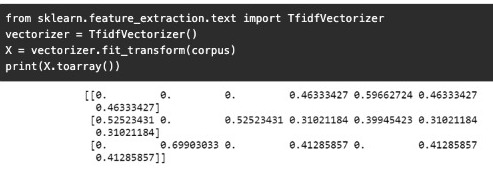
\includegraphics{vector.jpeg}
\end{center}
In the example above, text is added into the method and as a result we get vector, where its values are scores calculated for each word in the text.
\subsection*{STEP 3. Measuring similarity between two documents: }
After getting all the words converted into vector format, we apply similarity measurement method: $cosine_similarity$. Capturing the similarity of two documents using cosine similarity measurement. The cosine similarity is calculated by measuring the cosine of the angle between two document vectors. Using the formula: 
\begin{center}
    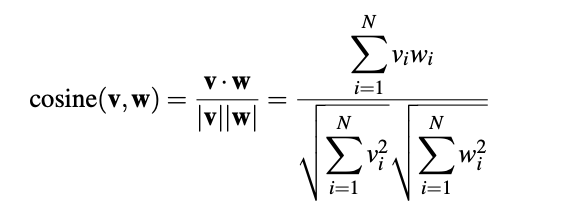
\includegraphics{formula.png}
\end{center}
\subsubsection{Cosine Similarity Measure}
The concept of similarity is fundamentally important in almost every field. Similarity is a core element in achieving an understanding of variables that motivate behavior and mediate affect. 
Cosine similarity is a measure of similarity between two vectors of n dimensions by finding the cosine of the angle between them, often used to compare documents in text mining. Given two vectors of attributes, A and B, the cosine similarity, is represented using a dot product and magnitude
as for text matching, the attribute vectors A and B are usually the tf vectors of the documents. The cosine similarity can be seen as a method of normalizing document length during comparison.
In \hyperlink{thisimage}{this image} it is illustrated how we applied the method in our implementation.\\
In the case of text retrieval, the result of cosine similarity will be between 0 and 1. If the result is closer to 1 (one), then it means the second document is significantly matching with the  reference
document.


    \chapter{Future roadmap & iterations}\label{ch:C}
Planning new functionalities to add:\\
1. Integrate bonuses systems, powered with AI
2. Export grades by data range : grade book\\
3. Integrate Chat bot\\
4. Post one assignment into several classes in one time: (one-to-many)\\
5. Pin an essential message in the platform\\
6. Tutorials on how to use a platform
    
    

    \chapter{Discussion}\label{ch:disc}
We faced some issues during implementation like not knowing how to concretize questions aiming to get to the point answers in an effort to shape our vision of a product. We worked in a flexible manner conforming to Agile methodology. It was the right decision we made because during the development phase no one amendments were made to the platform. For instance, we didn't plan to add timer feature, didn't target to add block of text with motivational citates and useful information. But later these features were added after we started to receive responds backing up these ideas. Now, about what we removed. In the third phase of our work, we decided to focus more on student's side rather than on teacher's, finishing up teacher's role just with basic functions. This happened because the way we wanted to implement plagiarism check function was too cumbersome and out of frame of our knowledge, thus it took a lot of our backend developer's time to realize this and we decided to apply our well-known methods using python libraries.    
However, tackling all these issues one by one as a team, brainstorming and making decisions together, we could overcome it. 
As a result, now we can answer the questions that arose in our minds before doing our research:\\
\textbf{What additional opportunities do teachers and children need during the work with domestic online platforms? } \\
* to view syllabys of a subject in advance\\
* to leave comments on student's work\\
* to get statistics about plagiarism\\
* to create classes on the platform\\
* to view overall progress visually\\
* to bind learning process with bonuses system\\
\textbf{What functions are hard to be found in the online education environment?}\\
* to view syllabys of subject in advance\\
* to upload the work\\
* to view assignments\\
* old design\\
\textbf{How to improve the level of productivity of school children?}\\
* by providing clear expectations and instructions\\
* by providing teacher-created videos \cite{bond2020facilitating}.\\

    \chapter{Conclusion}\label{ch:concl}
The purpose of this research was to create a useful, functional platform for schools, enriched with functionalities satisfying both teachers' and pupils' certain needs built in slight kazakh modern national style. Before coming up with this idea, we underestimated how worthy domestic platforms can be. There was an opinion like, there are already a lot of educational platforms, why do we need to create one more? However, as we wanted to maintain and upgrade our national values and as we became aware of issues that currently existing domestic and foreign platforms couldn't solve, we decided it is time to seize an opportunity. And we made a start on it. 

This research let us know that school pupils need an update in the online environment, both in the functionality and user interface experience context. To handle the situation we held questionnaires, interviews, where we've seen dissatisfaction with platforms to certain degree (rate 3.5 out of 5). For instance, leak in security, lack of plagiarism check, no overall view of progress opportunity. However, those are the essential aspects that should be taken into account during studying at school and gaining education in general. We've noticed the significance of this functions after interviewing, querying school pupils, teachers and university staff. 

During the implementation of platform we faced some obstacles during the development of frontend side, in a team with no frontend developer, it was a  challenge for us to combine backend part with frontend part. Nevertheless, our team members have a clear vision of our product's perspective and no hurdle made us stop. As a result we were able to integrate both parts. And we are proud of our work, of our team work strategy!

To conclude, we can say that we have created a useful, user friendly platform, which helps to maintain not only educational habits, but also helps to rise young generation's love to our national values. The viability of platform's functions were approved by teachers, school pupils, which instilled in us more faith and positive attitude towards the vision of our product. 

School is the place where children conceive an idea about gaining education as we mentioned in our introduction part (\cref{ch:intro}). And we feel that children's first impression in school should be as bright and joyfull as it is possible in order to pave the way for future innovations of today's young generation. And these innovations, of course, should be made in favor of our motherland. So, we believe that the platform is able to relief managing, studying, lesson organizing processes at schools by rising their love to our national language, style and worths. 


    
    \appendix
    \chapter{Additional data and tables}\label{app:A}
\section{Functional requirements}\vspace{0.3cm}
   \resizebox{\textwidth}{!}{%
    \begin{tabular} {|p{5cm}|c|p{7cm}|} %\begin{tabular}{|p{2cm}|p{5cm}|}  
    \hline
    What to \hypertarget{thistable}{do}? & User Story  \\
    \hline
    Login on mobile & As a new user, I want to sign up using my existing Google account so that I don't have to keep track of another account. \\
    \hline
    Functions for teacher & As a teacher, I want to create classes, add students to them, and assign them tasks/projects.\\
    \hline
    List of tasks/projects & As an existing student, I want to see all my tasks, so that I don't miss any of them. \\
    \hline
    Function for breaking down tasks & As a student, I want to break down assigned tasks, and prioritize them, so that I could work effectively. \\
    \hline
    View statistics & As a teacher, I want to see statistics on plagiarism, to make sure that evaluating process is fare. \\
    \hline
    Progress Tracking block & As a teacher, I want to see students' progress for specific data range. \\
    \hline
    Add timer page & As a student, I want to see time I spent on particular task, so that I can manage my energy and distribute my time wisely.\\
    \hline
    
    \end{tabular}
    }
\section{Images}
\hypertarget{thisimage}{Similarity measuring using python:}\newline
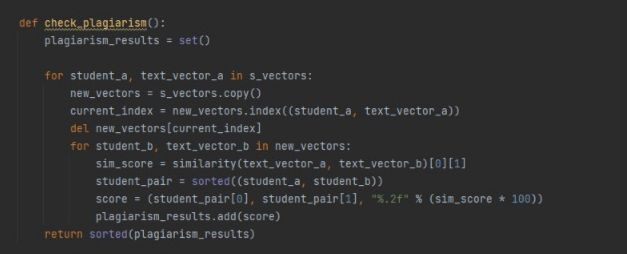
\includegraphics{code1.jpeg}

    \chapter{Phrases and acronyms}\label{app:B}
\textbf{INVEST} acronym:\\
Independent: Can the story stand by itself?\\
Negotiable: Can you change or remove this story without impacting
the rest of the project?\\
Valuable: Does this story have value to the end user?\\
Estimable: Can you estimate the size of the story?\\
Small: Is the user story small enough?\\
Testable: Can you test this story?\\
\hypertarget{thebag}{\textbf{Bag of words}} is a method to extract features from text documents. These features can be used for training machine learning algorithms. It creates a vocabulary of all the unique words occurring in all the documents in the training set.\\
\hypertarget{stopwords}{\textbf{Stopwords} are the words which do not add much meaning to a sentence, which are frequently occurring, insignificant words.}\\
\hypertarget{tfidf}{\textbf{TF} - Term Frequency, \textbf{IDF} - Inverse Document Frequency}

    \chapter{References}\label{ch:Ref}
\href{https://www.nu.edu/resources/challenges-of-distance-learning-for-students/}{(1)Challenges of online learning}\tab \url{https://www.nu.edu/resources/challenges-of-distance-learning-for-students/}\\
\href{https://www.capitalone.com/tech/machine-learning/understanding-tf-idf/}{(2)Why tf idf?}\tab \url{https://www.capitalone.com/tech/machine-learning/understanding-tf-idf/}\\
\href{https://lucidspark.com/blog/what-is-agile-methodology }{(3)Agile}\tab \url{https://lucidspark.com/blog/what-is-agile-methodology}
\href{https://cabar.asia/en/difficulties-of-transition-to-distance-learning-the-case-of-kazakhstan}{(4)Challenges of online edu}\tab \url{https://cabar.asia/en/difficulties-of-transition-to-distance-learning-the-case-of-kazakhstan}\\
\href{https://www.freecodecamp.org/news/an-introduction-to-bag-of-words-and-how-to-code-it-in-python-for-nlp-282e87a9da04/}{(5)Bag of words}\tab \url{https://www.freecodecamp.org/news/an-introduction-to-bag-of-words-and-how-to-code-it-in-python-for-nlp-282e87a9da04/}



    
    \bibliographystyle{plain}
    \printbibliography
\end{document}
